\section{Технологическая часть}

В данном разделе описываются средства разработки программного обеспечения, требования к вычислительной системе. Приводится структура разработанного приложения.

\subsection{Выбор средств разработки}

Из рассмотренных в аналитическом разделе трансляторов FEX лучше прочих подходит для реализации алгоритма, так как в нем присутствует СЕП.

\subsubsection{Выбор языка программирования}

Динамический транслятор FEX написан на языке C++, в нем используются разные библиотеки, например ядро транслятора FEXCore это библиотека реализующая непосредственно динамическую трансляцию. FEXCore также написан на C++ и не предусматривает расширений с помощью внешних модулей, поэтому для того чтобы ее модифицировать надо писать код на C++.

\subsubsection{Сборка программного обеспечения}

Для конфигурации проекта используется CMake. \cite{cmake} Для компиляции реализации алгоритма необходимо добавить имя файла в соответствующий \\ CMakeLists.txt.

Для сборки всего проекта используется ninja. \cite{ninja} На листинге \ref{code:args} указана конфигурация сборки проекта.

\begin{code}
	\captionof{listing}{Конфигурация сборки проекта}
	\label{code:args}
	\begin{minted}
		[
		frame=single,
		framerule=0.5pt,
		framesep=20pt,
		fontsize=\small,
		tabsize=4,
		linenos,
		numbersep=5pt,
		xleftmargin=10pt,
		]
		{text}
CC=clang CXX=clang++ cmake -DCMAKE_INSTALL_PREFIX=/usr \
-DCMAKE_BUILD_TYPE=Release -DENABLE_LTO=True \
-DBUILD_TESTS=False -DCMAKE_CXX_COMPILER_LAUNCHER=ccache \
-DENABLE_CLANG_FORMAT=False -G Ninja ..
	\end{minted}
\end{code}

Оптимизирующий проход создан на основе версии 2204, коммит \\ 37f1e55ed5dc7a35ba9bf875e250de0b75581a22.

\begin{figure}[hbtp]
	\centering
	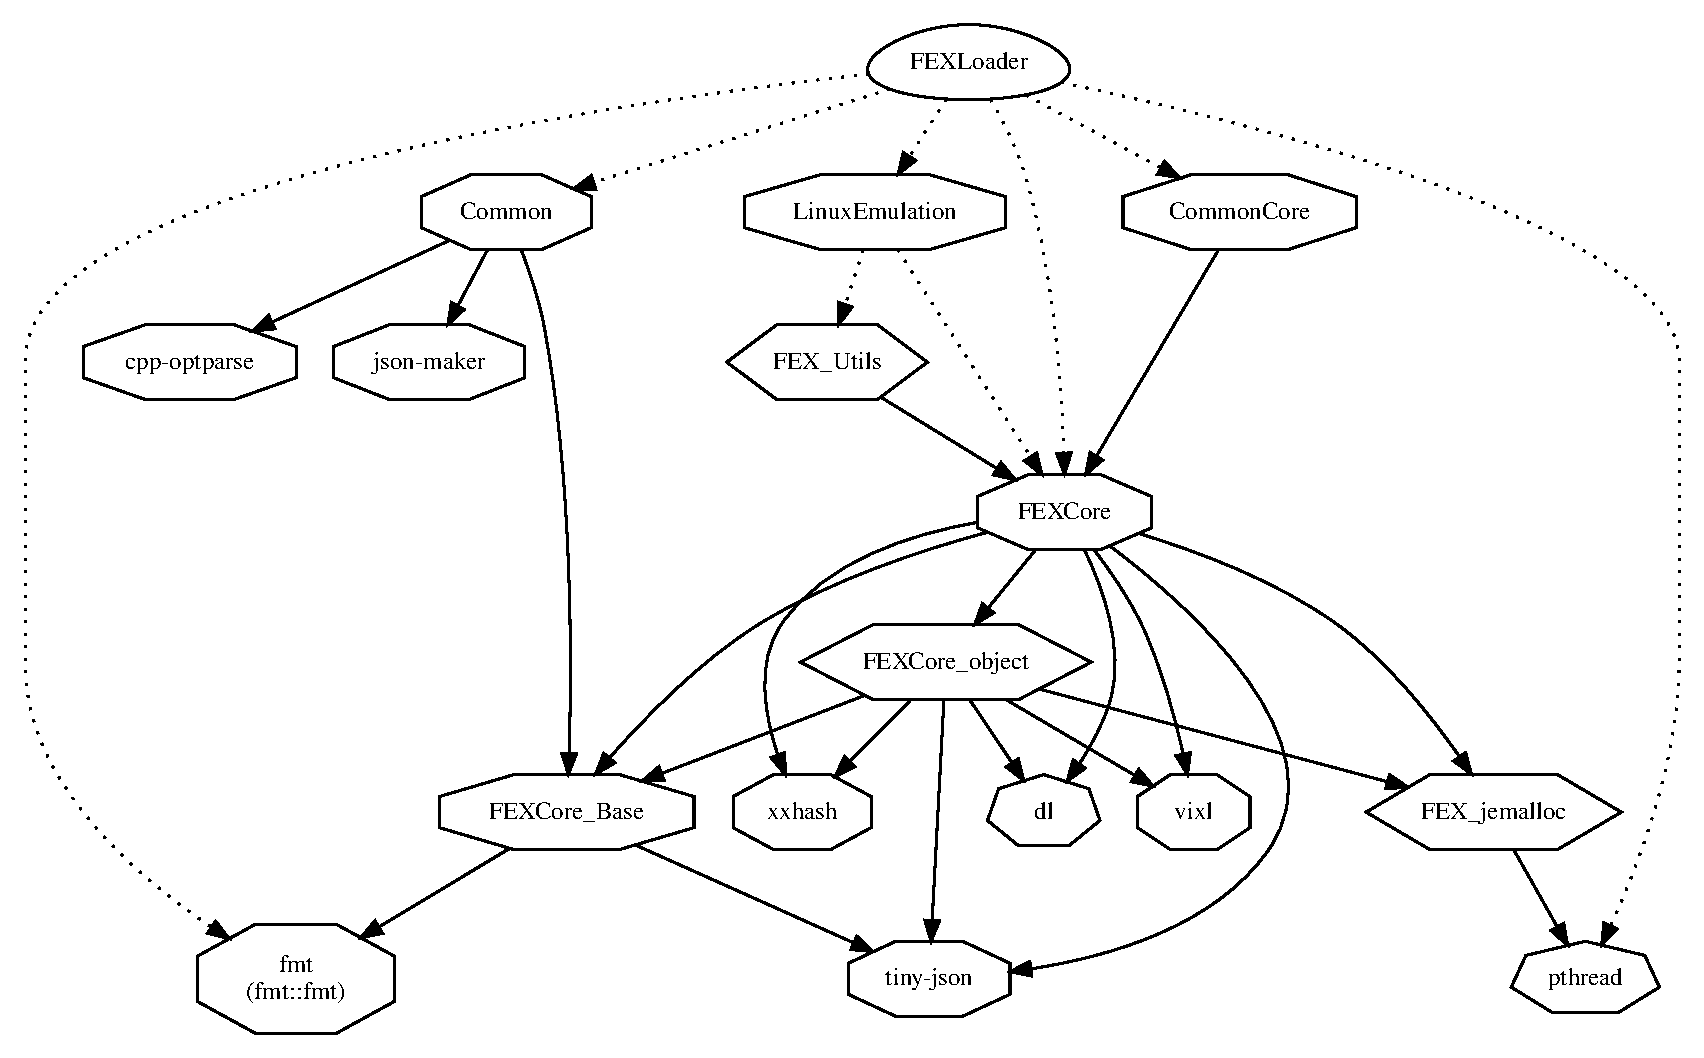
\includegraphics[width=\textwidth]{img/loader.eps}
	\caption{Диаграмма зависимостей userspace эмулятора FEXLoader}
	\label{fig:box64sig}
\end{figure}

Вносимые в проект изменения относятся к FEXCore\_Base.

\subsection{Требования к вычислительной системе}

Для запуска программного обеспечения требуется исходный код динамического транслятора FEX. Так как алгоритм реализует оптимизацию доступа к памяти с сохранением корректного выполнения многопоточных приложений для прироста в скорости требуется процессор с поддерживаемой архитектурой со слабым доступом к памяти и несколькими ядрами, то есть оптимизирующий проход будет приводить к росту производительности не только на ARM, но и, например, RISC-V.

Для разработки и сборки проекта использовался ноутбук на основе процессора RK3399, архитектуры ARM. Несмотря на это разработка не привязана к конкретной архитектуре, теоретически разработку можно вести на любой архитектуре имеющий набор инструментов для кросс-компиляции под архитектуру ARM.

\subsection{Структура программного обеспечения}

Разработанное ПО реализовано как оптимизирующий проход над промежуточным представлением.

При инициализации транслятора вызывается функция AddDefaultPasses, внутри которой вызываются функции InsertPass регистрирующие оптимизирующие проходы в определенном порядке. Функция InsertPass принимает на вход std::unique\_ptr<Pass> --- указатель на экземпляр класса прохода. У класса обязательно должен быть метод Run принимающий на вход IREmitter и возвращающий bool --- был ли изменен код во время прохода.

Разработанный проход зависит от StaticRegisterAllocationPass, во время этого прохода статически выделяются регистры, на основе этих регистров и идет оптимизация доступа памяти.

Отключить все оптимизирующие проходы можно с помощью аргумента -O или --o0.

\subsection{Распространение программного обеспечения}

Программное обеспечение распространяется в виде патча сформированного командой git format-patch. Для применения патча к проекту можно, например, использовать git am.

\subsection{Дополнительные утилиты}

Для анализа генерируемого кода нужно анализировать скомпилированный код, такой возможности у FEX нет, поэтому была проведена модификация функции Context::CompileBlock которая компилирует и запускает блок. Перед запуском вся область запускаемой памяти сохраняется в бинарный файл.

\newpage

\begin{code}
	\captionof{listing}{Сохранение скомпилированного блока}
	\label{code:args}
	\begin{minted}
		[
		frame=single,
		framerule=0.5pt,
		framesep=20pt,
		fontsize=\small,
		tabsize=4,
		linenos,
		numbersep=5pt,
		xleftmargin=10pt,
		]
		{text}
--- a/External/FEXCore/Source/Interface/Core/Core.cpp
+++ b/External/FEXCore/Source/Interface/Core/Core.cpp
@@ -1001,6 +1001,15 @@ namespace FEXCore::Context {
}
}

+
+    FILE *fp;
+
+    std::string filename = "Core_Block_other_" + \ 
+      std::to_string((uint64_t)CodePtr) + ".cdmp";
+    fp = fopen(filename.c_str(), "wb");
+    fwrite((void*)CodePtr, DebugData->HostCodeSize, 1, fp);
+    fclose(fp);
+    printf("block dumped %s\n", filename.c_str());
+
if (IRCaptureCache.PostCompileCode(
Thread,
CodePtr,
-- 
2.36.0

	\end{minted}
\end{code}

Обработка сохраненной памяти затем выполнялась при помощи objdump \cite{objdump} --- в итоге получался код на ассемблере.

После анализа скомпилированного кода были сделаны выводы по основным факторам замедляющим выполнение скомпилированного кода, таких как барьерный доступ к памяти.

\begin{comment}
\subsection{как контрибьютить}

Ведущими разработчиками являются такие то, чтобы пропихнуть патч надо то-то. Требуется одобрение такого то.
\end{comment}

\subsection{Методы оптимизирующего прохода.}

Всего реализовано 4 метода класса: Run, CalculateControlFlowInfo, \\ CalculateComplexState и HitsRegister.

\begin{table}[!htb]
	\label{table:benches}
	\begin{center}
		\caption{Методы оптимизирующего прохода.}
		\begin{tabular}{|c|p{4.5cm}|p{5.5cm}|}
			\hline
			\bfseries Метод & \bfseries Параметры & \bfseries Описание \\
			\hline
			Run & IREmitter* IREmit & Убирает барьерный доступ к памяти стека \\ \hline
			CalculateControlFlowInfo & IREmitter* IREmit & Строит граф потока выполнения блоков \\ \hline
			CalculateComplexState & OrderedNode* TargetNode,
			IRListView\& CurrentIR & Рассчитывает состояние регистра в блоке с учетом предшественников \\ \hline
			HitsRegister & int Register, IREmitter* IREmit,
			IROp\_Header* Op & Проверяет, связано ли значение в IROp\_Header с адресом стека \\ \hline
		\end{tabular}
	\end{center}
\end{table}

%диаграмма функциональная типа функции кто кого вызывает

На листингах \ref{code:blockinfo}-\ref{} представлены реализации описанных в конструкторской части структур данных.

\begin{code}
	\captionof{listing}{Структуры данных использующиеся в оптимизирующем проходе}
	\label{code:blockinfo}
	\begin{minted}
		[
		frame=single,
		framerule=0.5pt,
		framesep=20pt,
		fontsize=\small,
		tabsize=4,
		linenos,
		numbersep=5pt,
		xleftmargin=10pt,
		]
		{text}
enum RBP_STATE {
	NOT_CHANGED = (0b000 << 0),
	STACK = (0b001 << 0),
	NOT_STACK = (0b010 << 0),
};

struct BlockInfo {
	int State = NOT_CHANGED;
	std::set<OrderedNode*> StackNodes;
	std::set<OrderedNode*> UnStackNodes;
	std::vector<OrderedNode*> Predecessors;
	bool Visited = false;
};

std::unordered_map<NodeID, BlockInfo> OffsetToBlockMap;
\end{minted}
\end{code}

\begin{code}
	\captionof{listing}{Реализация OrderedNode в FEX}
	\label{code:blockinfo}
	\begin{minted}
		[
		frame=single,
		framerule=0.5pt,
		framesep=20pt,
		fontsize=\small,
		tabsize=4,
		linenos,
		numbersep=5pt,
		xleftmargin=10pt,
		]
		{text}
struct OrderedNodeHeader {
	OpNodeWrapper Value;
	OrderedNodeWrapper Next;
	OrderedNodeWrapper Previous;
};
		
class OrderedNode final {
	friend class NodeWrapperIterator;
	friend class OrderedList;
	public:
	OrderedNodeHeader Header;
	uint32_t NumUses;
		
	...

};
	\end{minted}
\end{code}

\subsection{Вывод}

В данном разделе были описаны средства разработки программного
обеспечения, требования к вычислительной системе. Была дана структура
разработанного приложения.

\pagebreak